% Figures in this chapter
\newcommand{\Tasks}{1}
\newcommand{\StimOutcome}{\Tasks A}
\newcommand{\StimAction}{\Tasks B}
\newcommand{\FeatureRelevance}{\Tasks C}

\newcommand{\Mechanisms}{2}
\newcommand{\LTP}{\Tasks A}
\newcommand{\TopDown}{\Tasks A}

\chapter{The role of sensory cortex in behavioral flexibility}

\section{Author contributions}
\noindent Lan Guo, Nicholas D Ponvert, and Santiago Jaramillo, 2017. The role of sensory cortex in behavioral flexibility. \textit{Neuroscience} 345: 3-11. 
%
Santaigo Jaramillo provided mentorship for all aspects of the study. Lan Guo, Nicholas D. Ponvert, and Santiago Jaramillo wrote the sections of the paper included in this dissertation.


%%%%% No abstracts inside chapters!
%% \section{Abstract}
%% To thrive in a changing environment, organisms evolved strategies for rapidly modifying their behavioral responses to sensory stimuli. In this review, we investigate the role of sensory cortical circuits in these flexible behaviors. 
%% %
%% First, we provide a framework for classifying tasks in which flexibility is required. We then present studies in animal models which demonstrate that responses of sensory cortical neurons depend on the expected outcome associated with a stimulus. Last, we discuss inactivation studies which indicate that sensory cortex facilitates behavioral flexibility, but is not always required for adapting to changes in environmental conditions.
%% %
%% This analysis provides insights into the contributions of cortical and subcortical sensory circuits to flexibility in behavior.

\section{Introduction}
Behavioral flexibility is defined as the ability to shift response patterns (or strategies) after changes in environmental conditions \citep{Ragozzino2007}. These environmental conditions define the statistical relations between a stimulus, possible behavioral responses, and outcomes (such as a rewards or punishments). We refer to these relations as \emph{contingencies}. 
%
The ability to adapt to changing contingencies is impaired in several human neurological disorders, including schizophrenia \citep{Goldberg1988,Morice1990} and autism \citep{Hill2004}. Our quest to develop better diagnostic and therapeutic strategies for these disorders would greatly benefit from detailed knowledge of the circuits and mechanisms responsible for flexibility in behavior.
%
Research on the neural basis of flexible behaviors in mammals has identified regions of the frontal cortex that detect changes in contingencies, inhibit undesired responses, and help acquire new strategies \citep{Dias1997,Ragozzino2007, Sotres-Bayon2010}. In contrast, it is not clear whether sensory cortex plays a role in implementing flexibility in behavior beyond extracting features of sensory stimuli. 

Understanding the neural mechanisms underlying flexible behaviors, and the role of sensory cortical neurons, requires monitoring neuronal activity with single cell resolution and manipulating the system in ways difficult to achieve in human subjects. For this reason, we focus here on experiments that use animal models of flexible behaviors.
%
We review studies in which sensory neurons are monitored or manipulated during changes in contingencies to address the following questions: What roles do sensory pathways play in behavioral flexibility beyond conveying sensory information? What flexible behaviors require sensory cortex? Which subcortical pathways can implement flexible behaviors without the need of the sensory cortex?

Several parallel neural pathways link sensation to action, including circuits in the brainstem that mediate reflexive responses, subcortical circuits via the amygdala that can mediate fear responses, and higher-order pathways that rely on sensory and motor cortex. In this review, we investigate how a stimulus can drive different behavioral responses depending on environmental conditions. A neuronal population within a sensory pathway can play at least three different roles during flexible behaviors. First, these neurons may be the first stage in the ascending sensory pathway that can discriminate the stimuli presented in a task. These neurons will be required for successful performance of the task, even though they do not play a direct role in rerouting information upon a contingency change. Second, this population may be the first stage in the ascending pathway that can communicate with circuits that reroute signals to implement behavioral flexibility. In this case, even though other regions (closer to the periphery) may be able to discriminate the stimuli in the task, information has to go through this specific stage before it can be flexibly rerouted to drive distinct actions.
% 
Third, a population of sensory neurons may play an active role in signal rerouting---passing or filtering out signals depending on the desired behavioral outputs for a given contingency. In this last scenario, we say that these neurons take part in implementing flexibility. 
%
Brain regions can play one or more of these roles, and do so in the context of coordinated activity across multiple other regions.

Here we review studies that quantify the correlations between sensory neural representations and behavioral contingencies. These studies indicate that sensory representations are modulated by expected outcomes associated with a stimulus, and when animals selectively attend to relevant stimulus features.
%
In addition, we discuss the behavioral effects of manipulating neural activity in sensory cortex during tasks that require flexibility. Sensory cortex lesions often impair behavioral adaptation following contingency changes. However, some flexible behaviors are possible after inactivation of sensory cortex.

\section{Taxonomy of adaptive behaviors}
%
In this section, we provide a framework for classifying different types of adaptive and flexible behaviors according to the relations between sensory stimuli, behavioral responses, and outcomes (such as rewards or punishments). We start by discussing phenomena in which these relations do not change, yet the nervous system can adapt to the statistics of a stimulus ensemble. We then discuss phenomena in which these relations do change, and classify these phenomena into three categories of flexible behaviors.

Neural correlates of adaptation to stimulus ensemble statistics can be observed even in anesthetized animals, and occur independently of reward contingencies. Examples include changes that result from contrast adaptation in the retina \citep{Baccus2002} and from adaptation to repetitive acoustic stimuli observed in the midbrain \citep{Malmierca2009}, thalamus \citep{Anderson2009} and cortex \citep{Ulanovsky2003}. 
%
In behaving animals, this adaptation provides a performance advantage by allocating neuronal resources to maximize the detection or discrimination of stimuli.
%
Some cases of \emph{perceptual learning}, defined as the improvement in sensory discrimination by practice \citep{Goldstone1998}, are examples of this type of adaptation without changes in reward contingencies. For instance, auditory cortical circuits change their sound frequency tuning as animals are trained to discriminate small differences in the frequency of sequentially presented tones \citep{Recanzone1993}.
%
In addition, subjects can use selective attention in tasks where the stimulus-action-outcome associations do not change.
In this case, subjects allocate resources to space \citep{Posner1980} or time \citep{Jaramillo2011} in order to improve task performance, resulting in changes of sensory cortical neural responses.
%
In all these scenarios, the relation between the stimulus, action and outcome does not change, and the only environmental feature driving adaptation is the stimulus ensemble. We exclude these phenomena from our discussion of behavioral flexibility. 

Here we focus on a different class of phenomena in which adaptation is driven by changes in the statistical relation between stimuli, behavioral responses and outcomes, \emph{i.e.}, changes in behavioral contingency. We first discuss scenarios in which the outcome associated with a stimulus varies across contingencies, as illustrated in \fig{\StimOutcome}. In this example, the star stimulus predicts a rewarding outcome in one condition (C1), but not in the other (C2). The circle stimulus, in contrast, is not associated with any outcome in the initial condition, but predicts reward when the contingency changes.
%
In this class of phenomena, which include acquisition and extinction of conditioned responses, actions may not be required to trigger a reward or punishment.

In the second type of scenario discussed, animals are required to change the action associated with a stimulus, but the outcome that can be achieved for each stimulus remains the same. 
%
This is illustrated with the discrimination task in \fig{\StimAction}. To obtain reward after a stimulus is presented, the subject must perform one of two possible actions: move right (R) or left (L). In the initial contingency (C1), the star stimulus predicts that the subject will obtain reward only after action R, while the circle predicts reward for action L. In contingency C2, the actions that yield reward for each stimulus are reversed. In contrast to the scenario described in \fig{\StimOutcome}, both stimuli predict reward under all contingencies in this task.
 
Separately, we discuss a special case of reversal phenomena in which selective attention can be used to filter out some features of the stimulus (\fig{\FeatureRelevance}).
%
During stimulus-driven behaviors, not all features of the environment are relevant at all times, \emph{i.e.}, some features may not predict outcomes. Depending on how the relevance of stimulus features changes across contingencies, we can define two different types of tasks. In the reversal task presented in \fig{\StimAction}, irrelevant features of the stimulus (such as the background in which it is presented) never become relevant. In contrast, parts of the stimulus in the task presented in \fig{\FeatureRelevance} change from being predictive of reward to being irrelevant. In this scenario, it can be advantageous for the organism to filter out a different set of irrelevant features in each contingency by engaging selective attention. The right panel of \fig{\FeatureRelevance} illustrates the advantage provided by attention. In a task defined by a contingency table with 16 entries (8 for each of the two contingencies), an animal would need to learn all possible combinations to maximize performance. Alternatively, the animal could learn that under each contingency, only half of the stimulus is predictive of reward. Thus, if the animal can filter out the irrelevant half of the stimulus under each condition, only 4 entries must be learned to successfully perform the task. In the next sections, we review studies that monitor or manipulate sensory representations during these three types of flexible behaviors.

%%%%%%%%%%%%%%%%%%%%%%%% Figure Tasks %%%%%%%%%%%%%%%%%%%%%%%%%%%%%
\begin{figure}[hp]
  \begin{center}
    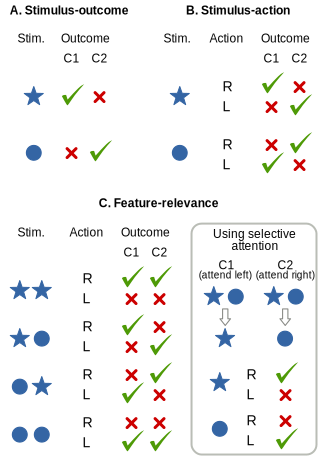
\includegraphics[height=5in]{figures/chapter5/figure_tasks}% 
  \end{center}
\caption{Types of flexible behaviors.}{Each panel shows the contingency table for a different type of task. The presence of an outcome, such as a reward, is indicated with a green check mark. A red cross mark indicates no outcome. \textbf{(A)} A task in which each stimulus (Stim.), either a star or a circle, presented in isolation predicts reward during one contingency (C1 or C2) but not the other. \textbf{(B)} A reversal task in which the possible outcomes for each stimulus remains the same, but the action, right (R) or left (L), required to obtain each outcome changes across contingencies. \textbf{(C)} A task in which a pair of items is presented simultaneously, but only one location is predictive of reward in each contingency. Animals can solve this task either by learning the full contingency table (left) or by using selective attention to filter out irrelevant regions/features of the stimulus (right box top) and applying a simpler contingency table for individual items (right box bottom). 
}
\end{figure}
%%%%%%%%%%%%%%%%%%%%%%%%%%%%%%%%%%%%%%%%%%%%%%%%%%%%%%%%%%%%%%%%%%%%%


\section{Stimulus representations in sensory cortex are modulated during flexible behaviors}

Do the responses of neurons in sensory pathways change depending on behavioral contingency? 
%
To address this question, we review studies that examine the neural representations of sensory stimuli before and after changes in stimulus-outcome associations (as in \fig{\StimOutcome}), stimulus-action associations (\fig{\StimAction}), and during flexible tasks in which animals can use selective attention to increase performance (\fig{\FeatureRelevance}).
%
We first present evidence that neural responses in stages as early as the sensory midbrain are influenced by the outcome associated with a stimulus.
%
These modulatory effects are present in a smaller percentage of sensory neurons if animals are required to modify their behavior in response to a stimulus, but the amount of reward (or punishment) associated with the stimulus remains the same.
%	
Last, we show that in tasks where features of the stimulus change relevance under different contingencies, attentional processes can strongly modulate sensory representations.

\subsection{Stimulus-outcome associations affect sensory representations}

Manipulation of stimulus-outcome associations can be achieved in the laboratory via several procedures including classical conditioning and extinction of conditioned responses. In classical conditioning, presentation of a conditioned stimulus (CS) is followed by either a punishment or a reward. Animals learn to associate this previously neutral stimulus with the outcome such that after conditioning the CS itself can elicit a conditioned response. This type of learning strongly modulates stimulus-evoked neural activity in sensory pathways. For instance, in the auditory system, these effects are evident in the midbrain, the medial division of the medial geniculate nucleus of the thalamus (MGm), primary auditory cortex (A1) and secondary auditory cortex (A2) \citep[reviewed in][]{Weinberger1987, Weinberger1993}, with sensory cortex neurons displaying longer-lasting modulation than midbrain and thalamic neurons \citep{Suga2003, Weinberger2007}. The firing rate of a large fraction of sound-responsive neurons in the MGm (71\% of cells), A1 (63\%), and A2 (95\%) is significantly modulated by the acquisition of a stimulus-outcome association in the cat \citep{Ryugo1978, Weinberger1984, Diamond1984}. In these experiments, MGm neurons showed 20-30\% changes in firing rate, whereas larger firing rate changes were observed in the cortex: 200-300\% change in A1 and 50-150\% in A2 \citep{Ryugo1978, Weinberger1984, Diamond1984}. In addition to changes in the size of evoked responses, altering stimulus-outcome associations modulates the receptive field properties of up to 75\% of auditory cortical neurons \citep{Fritz2003} and up to 60\% of inferior colliculus neurons in ferrets \citep{Slee2015}. 

Conditioning-induced increases in evoked neural activity are reversed during extinction of conditioned responses, \emph{i.e.}, when repeated presentation of the CS without reinforcement results in a decrease in the conditioned response.
In one study, auditory- and visual-responsive neurons in posterior thalamic nuclei that project to the amygdala and striatum in addition to sensory cortex showed responses to CS predictive of reward, with response amplitude proportional to the reward size \citep{Komura2001}. The sensory responses in these thalamic neurons decreased in amplitude or disappeared during extinction of the stimulus-reward association, and responses were again potentiated during reinstatement of reward. Separate studies showed that enhanced neuronal responses to a CS in the auditory cortex and the thalamus were reduced when the CS no longer predicted outcome \citep{Gabriel1976, Edeline1990}. 
Moreover, the area of auditory cortex responsive to the CS expands following conditioning and contracts following extinction, and the degree of contraction is correlated with the strength of extinction measured behaviorally \citep{Bieszczad2012}.
Overall, studies using conditioning acquisition and extinction reveal that stimulus-outcome associations modulate responses in sensory structures from midbrain to cortex in a reversible manner.

\subsection{Stimulus-action associations influence only a minority of sensory neurons}

In a different set of studies, the action required to obtain reward (given a stimulus) changed, but the amount of reward remained the same.
%
For example, a rhesus monkey was trained to perform an auditory discrimination task where a tone or a noise stimulus required shifting a lever left or right, respectively, to obtain reward. The stimulus-action contingency was then reversed, while the sound-evoked responses from the auditory cortex were measured. Although the majority of single-units recorded in the auditory cortex showed sensory-evoked responses, only 17\% of the sensory-responsive neurons showed responses modulated by the stimulus-action contingency \citep{Vaadia1982}. A separate study in rats found a similar modulation of evoked responses from both cortical and thalamic auditory neurons \citep{Jaramillo2014a}. Animals were trained to categorize sounds as low- or high-frequency by choosing the left or right reward ports of a training chamber after the presentation of a stimulus \citep{Jaramillo2014b}. The categorization boundary that separated low- from high-frequency sounds was shifted several times within each behavioral session, requiring animals to change the action associated with some stimuli. In this task, the reward given for a correct response was always kept constant. Therefore, the stimulus-outcome association remained the same throughout the task, while the stimulus-action association changed from one block of trials to the next. Only 15\% of responsive auditory cortical neuronsc and 16\% of responsive thalamic neurons were modulated by changes in the stimulus-action association. 
%
These studies suggest that a smaller percentage of neurons in sensory cortex and thalamus are modulated by changes in the behavioral response associated with a stimulus than by changes in the magnitude of reward. It is still possible that such a small percentage of cells can have an effect on behavior.

\subsection{Selective attention modulates sensory representations}

In some scenarios, subsets of features of a sensory stimulus that are initially relevant in predicting an outcome can become irrelevant. Subjects could solve these tasks by learning all relations between stimuli, actions and outcomes. A more efficient strategy requires using selective attention to filter out irrelevant features without the need for changing the associations between stimulus, actions and outcomes (\fig{\FeatureRelevance}).

The effects of attention on neuronal responses have been reviewed extensively \citep{Treue2001, Maunsell2002, Reynolds2004}. If two stimuli are presented within the receptive field of a neuron in the visual cortex, directing attention to one or the other stimulus strongly modulates the evoked activity in a large percentage of neurons. In area V4 of primates, 40-80\% of neurons display significant modulation of stimulus-evoked responses due to attention \citep{Motter1993, Luck1997, Reynolds1999, McAdams1999}, resulting in a 40-65\% change in firing rates \citep{Luck1997, McAdams1999}. Similar experiments show that roughly 80\% of cells in areas MT and MST are significantly modulated by attention, with a median firing rate modulation magnitude of about 80\% for MT and 100\% for MST \citep{Treue1996, Treue1999}. When two competing stimuli are far enough apart that they do not fall within the receptive field of a single neuron, the effects of attention are smaller, with only 13\% of V4 neurons displaying significant modulation \citep{Luck1997}. Roughly 50\% of neurons in areas MT and MST are modulated by attention under these conditions, with a median firing rate modulation of 19\% in MT and 40\% in MST \citep{Treue1996}. In addition to focusing attention on specific areas of visual space, subjects can direct attention to specific attributes of a stimulus. This type of feature-based attention also modulates the responses of visual cortex neurons \citep[reviewed in][]{Maunsell2006}. For instance, when monkeys were required to report the orientation of the stimulus that matched a color cue (and ignore all other stimuli), 74\% of V4 neurons displayed higher firing rate when the stimulus inside their receptive field matched the cued color compared to when a different color was cued. This effect of attention resulted in a doubling of the stimulus-evoked firing rate in these neurons \citep{Motter1994a}.

The effects of both spatial and feature-based attention have also been studied in the auditory system \citep{Fritz2007b, Hromadka2007}, although to a lesser extent. In an auditory-visual cross-modal attention task, roughly 67\% of stimulus-responsive neurons in the auditory cortex showed activity modulated by whether the monkey was required to respond to the light or respond to the sound \citep{Hocherman1976}. In human fMRI studies of multimodal attention, attending to one modality increased the response in the sensory cortical region corresponding to the attended modality and decreased activity in the sensory cortical region corresponding to the unattended modality \citep{Johnson2005}. Overall, these studies show that shifting attention largely modulates neuronal responses in sensory cortex.

\subsection{Summary of changes in sensory representations during flexible behaviors}
The studies reviewed in this section demonstrate that sensory neurons can integrate and represent stimulus relevance. Stimulus-evoked responses in over half of the recorded sensory neurons from areas in the midbrain to the cortex are modulated by changes in the outcome associated with a stimulus. This stimulus-outcome modulation is reversible on the same time scales as the behavioral changes. Moreover, changes in the relevance of stimulus features can engage attentional processes and result in modulation of sensory responses. In comparison, changing the action associated with a stimulus without changing the associated outcome yields modulation of responses in less than a fifth of neurons in sensory cortex and thalamus.

\section{Is sensory cortex required for behavioral flexibility?}

Correlational studies can reveal the environmental features that are represented in a brain region. However, manipulation studies are needed to provide information about the causal relationship between brain activity and behavior. 
Studies that inactivate sensory cortex find a wide range of effects on detection and discrimination of stimuli in audition \citep{Talwar2001, Rybalko2010, Gimenez2015, Kato2015} and vision \citep{Birch1978, Oakley1981, Glickfeld2013}. The largest effects are often seen for the discrimination of complex stimulus features, \emph{i.e.}, those not represented explicitly in the periphery \citep{Newsome1988, Ohl1999, Deutscher2006}. It is well established that selectivity for stimulus features of higher complexity increases in the ascending sensory pathways from the periphery to cortical regions \citep{Hubel1962, Miller2001a, Joris2004}.
%
When complex stimuli are used in a task, cortical lesion impairs discrimination performance, which makes it difficult to differentiate whether the cortex plays a role in implementing flexibility or simply transfers information to downstream structures that implement flexibility. Although animals are often exposed to stimuli of high complexity in their natural environments, experimental manipulations in the laboratory often use well-controlled simple stimuli in order to tease apart functional roles in stimulus processing versus roles in mediating flexible behavior.

\subsection{Sensory cortex facilitates extinction of stimulus-outcome associations} 


Studies that used aspiration or electrolytic lesions of sensory cortices before fear conditioning have found that acquisition of the conditioned fear response can still occur in the auditory \citep{Teich1989, Campeau1995, Song2010} and visual domains \citep{LeDoux1989, Falls1993}. 
%
Similarly, post-training excitotoxic lesions of the primary auditory cortex did not attenuate fear-potentiated startle in rats after 10 days of recovery \citep{Campeau1995}. 
%
However, more extensive post-training electrolytic lesions spanning secondary auditory and perirhinal cortex blocked fear memory recall, at least for the periods tested \citep{Campeau1995, Boatman2006}. Additional evidence of a cortical role in associative learning comes from a study in which protein synthesis inhibitors were applied to the auditory cortex during conditioning to frequency-modulated sounds \citep{Kraus2002}. 
%
This manipulation impaired the speed of learning, although application of the inhibitors in well-trained animals did not impair recall of the conditioned behavior. 

The effects of sensory cortex lesions on the extinction of conditioned responses have also been inconsistent across studies \citep[reviewed in][]{Myers2002}. 
%
For example, one study found that complete aspiration lesions of the visual cortex 10 days before fear conditioning to a visual CS did not prevent subsequent extinction \citep{Falls1993}. Other studies that also used pre-acquisition lesions of sensory cortex found impairments ranging from a slowdown of extinction \citep{Song2010} to a complete inability to extinguish the conditioned response for the periods tested \citep{LeDoux1989, Teich1989}.
%
Under some task conditions, pre-acquisition lesions of auditory cortex can severely impair the ability to respond flexibly to changing sound-outcome associations \citep{Ono2006}.
%
In these conditions, it appears that the impairment was not in the extinction of acquired associations, but either in the ability to form new associations or to respond to only the rewarded stimulus.
%
Post-acquisition lesions of sensory cortex have also been shown to retard responses to changing stimulus-outcome associations. For example, when rats were trained to associate an increase in stimulus intensity (the CS) with a footshock, sensory cortex lesions after acquisition resulted in slower adaptation when the CS was changed to a decrease in stimulus intensity. These effects were observed in both the auditory and visual domains \citep{Delay1994}. 


If fear conditioning can still proceed in the absence of sensory cortex, what subcortical sensory pathways mediate this behavior? Inactivation studies have found that both thalamo-amygdala and cortico-amygdala pathways can transfer information about an auditory conditioned stimulus during fear learning \citep{Romanski1992, Campeau1995}. Involvement of the thalamo-amygdala connections in conditioning is also supported by observations of conditioning-induced plasticity in these synapses \citep{McKernan1997, Quirk1997, Maren2004}. Altogether, these results suggest that multiple parallel pathways are engaged in fear conditioning in the intact brain.


\subsection{Sensory cortex is not always required for reversal learning of stimulus-action associations}

The role of sensory cortex in reversal learning has been investigated by treating the auditory cortex of gerbils with enzymes that degrade the extracellular matrix \citep{Happel2014}. This procedure, which restores juvenile-like levels of plasticity \citep{Pizzorusso2002, Gogolla2009}, made animals faster at reversing the action associated with frequency-modulated sounds. These results suggest a causal role of cortical plasticity in the reversals of stimulus-action associations. 
%
Other studies, however, show that animals can perform reversals of stimulus-action associations after extensive lesions of sensory cortex.

A study in rats tested performance on a visual discrimination task 12-25 weeks after near complete ($>$95\%) removal of the entire neocortex.
%
Animals discriminated between a door that was marked with a horizontal grating and a door marked with a vertical grating, one of which signaled the presence of a food reward. Lesioned animals were only slightly slower than controls at learning this behavior. When the pattern that signaled the correct door was reversed, lesioned animals took longer than controls to learn the reversal but were eventually able to reach the same performance criterion (18 correct choices in a row) as control animals \citep{Oakley1981}.
%
Another study using a similar visual discrimination paradigm found that rats with posterior decortication six weeks before training were also slower at reversing learned associations than controls \citep{Birch1978}. In this study, lesioned rats were less impaired when they only had access to light intensity cues, compared to when they were exposed to all spatio-visual cues, suggesting that cortical involvement in reversal learning depends on stimulus complexity. 


In the studies presented above, animals received lesions before behavioral training. A recent study investigated the effects of lesions after animals had been extensively trained to perform a flexible sound categorization task \citep{Gimenez2015}. In this task, animals must reverse the action associated with a sound multiple times over the course of a single session.
%
Rats were able to switch the action associated with a spectrally-simple sound to obtain water reward, even on the first post-lesion session that tested reversals (3-5 days after the surgery). The number of trials to switch was comparable before and after lesion. 
%
In contrast, lesions of the auditory thalamus severely impaired the ability to discriminate sound frequencies in this task, therefore preventing the expression of the flexible categorization behavior. All together, these results suggest that subcortical outputs of the auditory thalamus are capable of mediating this behavior.

Compensatory plasticity in subcortical circuits could explain why animals in these studies were able to perform reversal learning after cortical lesions.
%
However, when well-trained rats were tested during reversible bilateral inactivations of auditory cortex using muscimol, they were still able to flexibly switch between the previously-learned sound-action associations \citep{Gimenez2015}. These results suggest that if compensatory mechanisms are involved, they may be fast-acting. 
%
Overall, sensory cortex does not always appear to be required for flexible tasks where the action associated with a stimulus must be modified.
\subsection{Ability to filter out distractors is impaired by lesions of sensory cortex}  

Evidence that areas of the visual cortex are necessary for shifting attention comes mostly from studies that evaluate the effect of distractors on visual perception in primates before and after lesions. For instance, aspiration lesions of area V4 after extensive behavioral training largely affected the ability to saccade to a target item immersed in an array of other similar items \citep{Schiller1991}, although the ability to detect this stimulus in isolation was minimally affected. Similarly, aspiration lesions of areas V4 and TEO impaired the animals' ability to detect changes in the orientation of a stimulus when surrounded by high-contrast distractors \citep{DeWeerd1999}. The effect was minimal when the stimulus was presented in isolation. These effects were replicated for detection of color changes, but were not present during detection of changes in motion \citep{DeWeerd2003}. Because neurons in areas V4 and TEO are highly selective to orientation and color, but less so to motion, these results imply that the ability to ignore distracting visual features depends on the neural substrate that processes the relevant feature in a given task. 
Impaired ability to filter out visual distractors has also been observed in human patients with brain damage to the temporal lobe \citep{Mendola1999} and at the temporal-occipital junction \citep{Gallant2000}.

Studies of cortical lesions in humans also suggest impairments in spatial attention during dichotic listening tasks \citep{Woods1993, Bellmann2001}. However, since lesions are not always restricted to the auditory cortex, the exact cause of behavioral deficits are difficult to determine. 

\subsection{What have we learned from lesion studies?}
The studies reviewed in this section provide insights into the possible roles played by the sensory cortex during flexible behavior, and help determine what subcortical sensory pathways can do in the absence of the cortex.
% 
In the intact brain, sensorimotor selection likely involves coordinated activity in multiple regions, such that inactivating any of these could lead to an impairment \citep{Du2011}. The studies reviewed here indicate that sensory cortex lesions slow down the extinction of learned stimulus-outcome associations, as well as the reversal of stimulus-action associations, but do not always preclude these behaviors. Sensory cortex seems to be essential for filtering out distractors during attention tasks. 

Negative results from cortical lesion studies cannot rule out cortical involvement in a given behavioral task. The existence of multiple parallel pathways, or the reorganization of sensory circuits (compensatory plasticity), are potential explanations for the ability to perform flexible behaviors after cortical lesions. Compensatory plasticity can come about either through the formation of new pathways or through adaptation of downstream areas to changes in their inputs. An example of compensatory plasticity can be seen from studies of amplitude-modulated (AM) sound discrimination. Serial lesions of bilateral auditory cortices in Mongolian gerbils with intervening training did not result in an impairment on discrimination performance for fast AM tones \citep{Depner2014}. In contrast, simultaneous bilateral ablations led to complete loss of AM discrimination in the same paradigm \citep{Deutscher2006}. Training after the first unilateral lesion potentially triggers compensatory plasticity in subcortical pathways, which could compensate for the loss of cortical function. 

The development of new tools to manipulate neuronal activity has made possible the transient inactivation of neuronal circuits on a millisecond time scale. Such acute inactivation can potentially diminish the confounding effects of compensatory plasticity. However, if we wish to know whether brain regions besides the sensory cortex have the capabilities necessary for mediating a behavioral task, long-lasting cortical inactivations may still be advantageous. Acute inactivation can lead to sudden perturbations of information in downstream structures. Due to this transient imbalance in the circuit, acute inactivation experiments could potentially overestimate the functions carried out by the affected cortex, and make it difficult to test the sufficiency of subcortical areas alone \citep{Otchy2015}.

\section{Conclusions and future directions}
This review set out to address the role of sensory cortex in flexible behavior and what subcortical pathways can do in the absence of the cortex.
%
In summary, changing the expected outcome associated with a stimulus largely modulates sensory representations. Under these conditions, cortical inactivation affects the extinction of these stimulus-outcome associations without disrupting the acquisition.
%
In comparison, a smaller percentage of sensory neurons are modulated when behavioral responses must change in response to a stimulus, but the outcome associated with the stimulus remains the same. In this case, lesions of sensory cortex either slow down or do not affect the ability to update stimulus-action associations.
%
In tasks where selective attention can be used to filter out irrelevant stimuli, sensory cortex lesions lead to impaired performance, consistent with the large modulation of cortical neuronal activity observed during these tasks.
%
These results will guide future investigation of selection mechanisms in neuronal pathways that link sensation to action. 

Flexibility in behavior can be implemented either by selection of stimuli or by selection of actions, via two (and possibly more) distinct neural mechanisms. First, feedback about outcomes can result in long-term changes in synaptic strength along the sensorimotor pathway, such that a stimulus is linked to its appropriate response under each contingency (\fig{\LTP}). Such long-term changes can be observed in the synaptic strength in brain slices from trained animals \citep{McKernan1997, Xiong2015}. Second, neural signals from outside the sensorimotor pathway can influence which sensory signals drive particular actions, without the need of synaptic changes in this pathway (\fig{\TopDown}). This mechanism has been shown to account for attentional modulation of neural activity \citep{Jaramillo2007}. 
%
It is possible that neural circuits employ both of these selection mechanisms in parallel to implement behavioral flexibility.

%%%%%%%%%%%%%%%%%%%%%%%% Figure Mechanisms %%%%%%%%%%%%%%%%%%%%%%%%%%%%%
\begin{figure}[hp]
  \begin{center}
    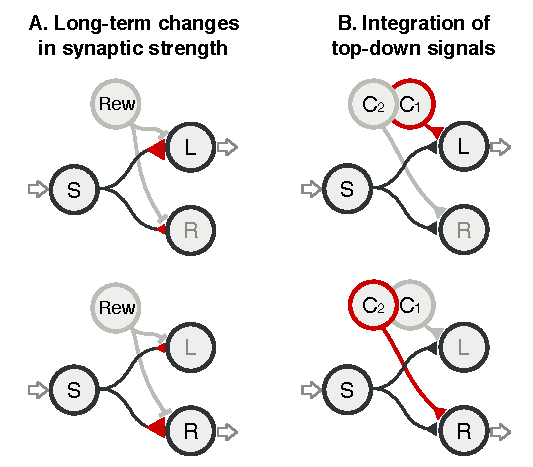
\includegraphics[height=4in]{figures/chapter5/figure_mechanisms}% 
  \end{center}
\caption{Two possible neuronal mechanisms for signal selection.}{Red indicates what changes in each scenario. \textbf{(A)} Signals from a sensory neuron (S) can be routed to drive different action neurons (R or L) by changing the synaptic strength of each pathway according to previous outcomes. In this scenario, reward-related signals (Rew) enable synaptic plasticity driven by the activity of pre- and post-synaptic neurons. The same sensory signal will drive action L (top) or R (bottom) depending on contingency. \textbf{(B)} Signals can also be routed without changes in synaptic strength in the sensorimotor pathway. In this scenario, top-down neurons that are selectively active in each contingency (C1 and C2) will bias which of the actions will be selected in response to sensory inputs. 
}
\end{figure}
%%%%%%%%%%%%%%%%%%%%%%%%%%%%%%%%%%%%%%%%%%%%%%%%%%%%%%%%%%%%%%%%%%%%%


How can we test which selection mechanism is recruited in the cortex during tasks that require behavioral flexibility? A first approach requires manipulating synaptic strength in competing sensorimotor pathways to test whether encoding of stimulus-outcome or stimulus-action associations is affected. For instance, induction of long-term potentiation and depression in cortico-amygdala and thalamo-amygdala synapses is sufficient to recapitulate the stimulus-outcome associations that result from classical conditioning \citep{Nabavi2014}. Similarly, manipulating potential sources of top-down signals can be used to test whether these signals are sufficient to drive sensorimotor selection, as has been done during visual selective attention \citep{Moore2003, Moore2004}. Lastly, blockade of plastic synaptic changes in sensorimotor pathways (without affecting synaptic transmission) can be used to test whether these changes are necessary for encoding stimulus-outcome associations \citep{Kraus2002, Quirk2008, Johansen2014}.
%
Using these tools, future studies can tease apart the conditions under which each of these two mechanisms is at play in sensory cortices. 
%
Impairments in behavioral flexibility observed in some neurological disorders \citep{Goldberg1988,Morice1990,Hill2004} could be the result of abnormalities in the components that regulate either of these selection mechanisms.  
%
Detailed knowledge of these mechanisms will inform development of effective treatment strategies for these disorders.


